\section{Agents as state machines}
\label{sec:machines}

Lecture~2 drew \msa{} as a state machine, and its Section~4 built a version of the agent with a
planner and a validator as a graph. This section makes that drawing precise by describing the agent
as an extended state machine, with control locations, variables and guarded transitions. We then
read a run as a path through a tree of possible runs and state what its trace records. These
definitions let us say which steps a run can take and why it ended, and which of those facts the
trace supports.

\Cref{sec:records} and \cref{sec:routing} show how the runtime, the code that runs the agent
(Lecture~2), stores the variables, chooses the next step and ends a run, and Lecture~4 covers how it
schedules and executes tools. \Cref{sec:discovery} and \cref{sec:triage} introduce the problem of the
first homework, HW1: deciding which alerts of a static-analysis scanner point to flaws that an
attacker can reach.

Our running example in this section and the next two is the \textbf{planning agent} of Lecture~2,
Section~4. It extends the reactive loop of \msa{} (Lecture~2, Section~3), in which the model chooses
each next action after reading the result of the previous one. The planning agent adds two nodes to
the loop: a planner, which writes the steps the run intends to take, and a validator, which decides
whether to accept a patch. Like the loop, it repairs one scanner alert at a time in OWASP
BenchmarkPython, the Python web application of Lecture~2, which is made up of many small test cases.

\subsection{A state machine as a description of an agent}
\label{sec:machines-description}

A state machine is a simplified description of an agent. It omits the prompts, the model and the
tool code, and it keeps only what decides how a run proceeds. An agent runs in discrete steps, such
as model calls, tool calls and checks. Between two steps the agent keeps some information, and the
program we wrote decides which stored values may change and which computation may run next.

Lecture~2 described a state machine as a set of states with transitions between them, and its
states were the agent's modes. In this lecture a state is the information the agent keeps between
steps, and \cref{sec:machines-locations} gives the modes their own name. A complete description of
a state machine has the following parts \citep[slide~17]{seshia2015discrete}:
\bi
\item \textbf{States.} The states are the values that the information kept between steps can take.
\item \textbf{Inputs.} The inputs are the results the agent can receive during a step.
\item \textbf{Outputs.} The outputs are what a step can emit, such as a request to run a tool.
\item \textbf{An initial configuration.} A configuration is the point a run has reached together
with the values of the information it keeps, as \cref{sec:machines-configurations} defines
precisely. The initial configuration fixes where every run begins and the values it begins with.
\item \textbf{A transition rule.} The transition rule specifies, for a state and an input, how the
state changes and what output the step produces.
\ei
A workflow that is meant to end also specifies where its runs end. These are the terminal
configurations of \cref{sec:machines-configurations}, from which the runtime schedules no further
step.

Because it leaves out the prompts, the model and the tool code, the description lets us examine how
the agent executes, which steps can follow which and when a run ends, without describing the whole
program. The model itself is not part of the description. Its replies enter the machine only as
inputs (\cref{sec:machines-state}).

\subsection{Control locations of the planning agent}
\label{sec:machines-locations}

A \textbf{control location} names the computation to run next, or marks the end of the run. In a
drawing of the machine, each control location is a node and each arrow is a \textbf{transition}, a
permitted step from one location to another. Lecture~2 called the Controller, Tool and Submit of
\msa{} its states. In this lecture they are control locations.

The planning agent has the following control locations (\cref{fig:machines-agent}):
\bi
\item \textbf{\demoref{plan}.} The planner calls a model to write the plan. It calls the model again
to revise the plan after the run stalls, which in Lecture~2 meant that three tool calls in a row
returned the same result. \Cref{sec:machines-planning} refines this condition.
\item \textbf{\demoref{controller}.} The controller calls a model whose reply either requests tools
or, by requesting none, proposes to submit.
\item \textbf{\demoref{tools}.} This location runs the requested tools, \demoref{read\_file},
\demoref{search} or \demoref{edit}, and records their results.
\item \textbf{\demoref{submit}.} This location runs three mechanical checks on the candidate patch:
that it applies, that it touches the line the alert flagged, and that a rescan of the patched code
no longer reports the alert.
\item \textbf{\demoref{validate}.} The validator calls a model that accepts or rejects the patch.
\item \textbf{\demoref{START} and \demoref{END}.} \demoref{START} runs no computation. It marks where
a run enters the machine, and the arrow from it gives the variables their starting values.
\demoref{END} marks the end of a run.
\ei
The locations \demoref{plan}, \demoref{controller} and \demoref{validate} call a model, and
\cref{fig:machines-agent} draws them in blue. The locations \demoref{tools} and \demoref{submit} run
tools or checks, and the figure draws them in grey.

\begin{figure*}[t]
  \centering
  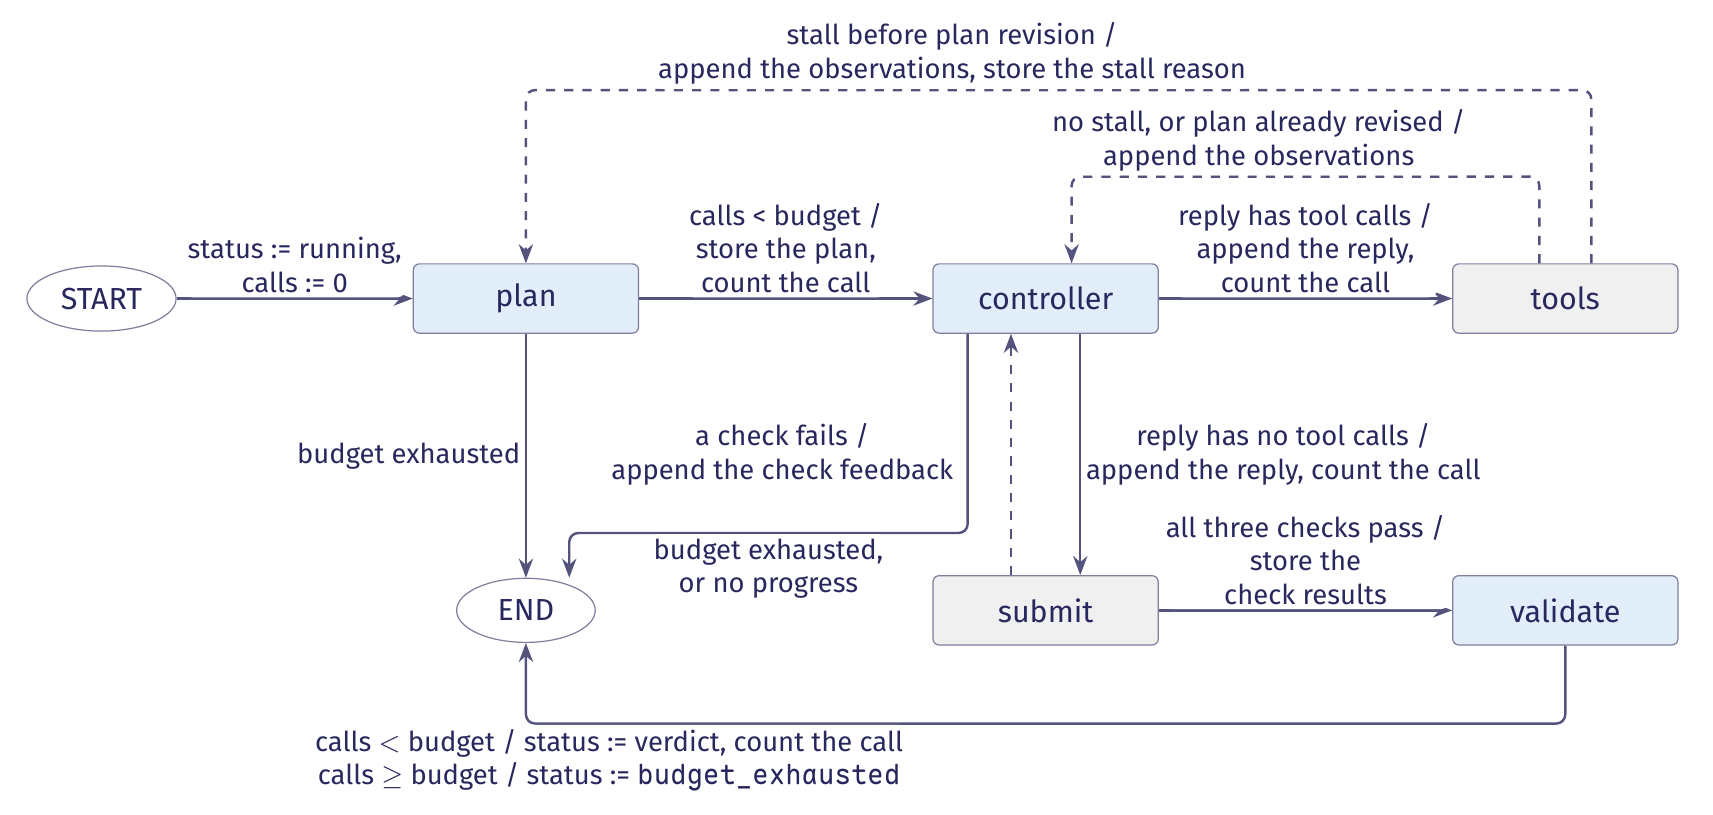
\includegraphics[width=0.92\textwidth]{figures/deck/675c3b4911.png}
  \caption{The planning agent as an extended state machine, with the nodes that call a model in blue
  and the nodes that run tools or checks in grey. Arrows carry guards and, after a slash, set
  actions, and the dashed arrows return to a location visited earlier.}
  \label{fig:machines-agent}
\end{figure*}

A run can visit the same location many times, and two visits to the controller can lead to
different next steps. What differs between the visits is the information the agent has kept, its
state.

\subsection{State, inputs and outputs}
\label{sec:machines-state}

The state of an agent is the information retained between steps that can affect what the agent does
next. Both the model and the runtime use that information. The controller's model reads its
instructions and the earlier observations, the results of tool calls as the runtime records them
(Lecture~2, Section~3), to choose an action. The runtime reads the call count, the number of model
calls made so far, to decide whether another model call is allowed.

\begin{definition}[State]
\label{def:machines-state}
State is the ``condition of the system at a particular point in time''. It ``[e]ncodes everything
about the past that influences the system's reaction to current input''
\citep[slide~10]{seshia2015discrete}.
\end{definition}

For an agent, the part of the past that reaches its next step through the state is what the agent
has kept: the messages exchanged with the model, the observations and the counters, among other
values. Anything else from the past can reach a later step only as an input.

An \textbf{input} is a result that the agent receives during a step: a model reply, a tool result
or the result of a check. The stored state alone does not determine an input. A model reply is an
input, so the same state can receive a different reply on another visit or in another run.

The files the agent works on lie outside the state in this description. The agent learns about them
through its tools and through the checks that \demoref{submit} runs. A tool's report about the files
enters the machine as an input, and the runtime then stores it as an observation. The result of an
edit, for example, records only that the edit was made, and a later read of that file reports the
new content.

An \textbf{output action} is the part of a transition that emits an output. The output is either a
request for an operation, such as running a tool, or the report of a terminal outcome, such as an
accepted patch.

The division between state and input separates what the program decides from what it receives. The
state determines which transitions are permitted. It does not determine which result arrives. Every
transition the agent can take is written in the program we designed, while the model, the tools and
the checks supply the inputs that select among them.

\subsection{Extended state machines and configurations}
\label{sec:machines-configurations}

An agent has a small number of control locations and a large amount of data, so we describe it as an
extended state machine. An \textbf{extended state machine} has finitely many control locations and a
set of variables that store data. Its transitions may read and write the variables.

\begin{definition}[Extended state machine]
\label{def:machines-extended}
``Extended state machines augment the FSM model with variables that may be read or written.''
\citep[slide~4]{seshia2015extended}
\end{definition}

In the quotation, FSM stands for finite-state machine, a state machine with finitely many states.

A \textbf{configuration} pairs the current control location with the current value of every
variable. It says where the run is and what the run holds. The variables hold the state of
\cref{sec:machines-state}. The configuration adds the control location, so one step can change the
location, the variables, or both.

For example, in the recorded run of \cref{sec:machines-trajectory}, just before the controller's
third model call, the configuration includes the following location and values:
\bi
\item \textbf{Location.} The run is at \demoref{controller}.
\item \textbf{\demoref{observations}.} Two tool results have been stored.
\item \textbf{\demoref{model\_calls}.} Three model calls have completed, one in \demoref{plan} and two
in \demoref{controller}.
\item \textbf{\demoref{status}.} The status is \demoref{running}. The status is the variable that
records whether the run is still going and, once it has ended, how it ended (Lecture~2).
\item \textbf{\demoref{messages}.} The variable holds the conversation so far.
\item \textbf{\demoref{plan}.} This variable, which shares its name with the location, holds the
plan: the list of steps the run intends to take. Lecture~2 called these steps plan steps, or
subgoals.
\ei
The configuration also holds the values of the other variables, such as the alert and the token
usage. In the same run, the controller is visited five times, and each visit has a different configuration
because the stored values have changed between visits.

Every run starts from the \textbf{initial configuration}. It pairs the first control location,
\demoref{plan}, with the starting values of the variables: the opening messages, counters at zero,
no observations and the status \demoref{running}. A \textbf{terminal configuration} is one from which
the runtime schedules no further step, so reaching it ends the run. The state then stores the reason
for ending, in the status.

An extended state machine can have finitely many control locations and infinitely many
configurations. How many configurations a location has depends on the values its variables can
take:
\bi
\item \textbf{A bounded counter.} The call budget, which Lecture~2 called the budget, is the most
model calls a run may make. If \demoref{model\_calls} were the only variable and the call budget were
$N$, the counter could hold the values $0$ through $N$. Each location would then have at most $N+1$
configurations, which is 41 for our budget of 40.
\item \textbf{An unbounded list.} If a list of messages can grow without a bound on its length, a
single control location can have infinitely many configurations.
\ei
A configuration is \textbf{reachable} when some run can arrive at it from the initial configuration.
When a machine has finitely many configurations, an analysis can examine every reachable one, for
example to show that no run arrives at an unsafe configuration. When a variable can take infinitely
many values, as the unbounded list can, a procedure that tries to list every reachable configuration
may never finish. The control locations and the guards (\cref{sec:machines-transitions}) still form
finite sets, and both are written in the program. An argument about the agent can therefore rest on
these finite sets and on properties of the variables, without listing configurations.
\Cref{sec:records} and \cref{sec:routing} argue in this way about the call budget.

\subsection{Transitions: guards, output actions and set actions}
\label{sec:machines-transitions}

In an extended state machine, a transition goes from one configuration to the next. Each transition
has a guard, an output action and a set action. The \textbf{guard} is a predicate, a true-or-false
test of the variables and the input, that states when the transition is allowed. The output action
emits the step's output (\cref{sec:machines-state}). The \textbf{set action} updates the variables.

Extended state machines label each arrow with the guard and the output action, separated by a slash,
and with the set action below them \citep[slide~5]{seshia2015extended}. We write one transition with
its input and the configurations before and after it:
\[
  (q, v) \xrightarrow{\;e\,;\; g \,/\, \mathit{out}\,;\, \mathit{set}\;} (q', v')
\]
At location $q$ with variable values $v$, input $e$ arrives. If the guard $g$ holds, the transition
emits $\mathit{out}$, applies $\mathit{set}$ to the variables, and moves to location $q'$ with values
$v'$.

\Cref{tab:machines-elements} gives each element of a transition its symbol and states what it is in
an agent. The guard is written $g(v, e)$ because it may test the stored variables, the new input, or
both.

\begin{table}[htbp]
  \caption{The elements of a transition in an agent's state machine, with the symbol used in the
  notation and what each element is in an agent.}
  \label{tab:machines-elements}
  \begin{adjustbox}{width=\linewidth}\begin{tabularx}{\linewidth}{L{0.24\linewidth}L{0.14\linewidth}X}
    \toprule
    \textbf{Element} & \textbf{Symbol} & \textbf{In an agent} \\
    \midrule
    \textbf{Control location} & $q$ & The computation ready to run: a model call, the execution of
      tools, or a check \\ \addlinespace
    \textbf{Variables} & $v$ & Messages, observations, a plan, counters, check results and a status,
      kept between steps \\ \addlinespace
    \textbf{Input} & $e$ & A result received during a step: a model reply, a tool result or a check
      result \\ \addlinespace
    \textbf{Guard} & $g(v, e)$ & A true-or-false test of the variables and the input, such as whether
      the reply requests a tool \\ \addlinespace
    \textbf{Output action} & $\mathit{out}$ & A request for an operation, or the report of a
      terminal outcome \\ \addlinespace
    \textbf{Set action} & $\mathit{set}$ & An update of the variables, such as storing a reply,
      extending the observations or incrementing a counter \\ \addlinespace
    \textbf{Initial configuration} & $(q_0, v_0)$ & The first control location with the starting
      values: opening messages, zero counters, no observations and the status \demoref{running} \\
      \addlinespace
    \textbf{Terminal configuration} & No symbol & A configuration from which no further computation is
      scheduled, with the reason for ending stored in the state \\
    \bottomrule
  \end{tabularx}\end{adjustbox}
\end{table}

The transition from the controller to the tools shows each element in code
(\cref{lst:machines-transition}). In the code, one transition is split between two functions. The
node \demoref{controller} receives the input and returns the set action. The routing function
\demoref{after\_controller} tests the guard. As in Lecture~2, Section~3, a routing function reads the
state after a node has finished and returns the name of the next location.

\noindent\begin{minipage}{\linewidth}
\begin{lstlisting}[basicstyle=\ttfamily\footnotesize, caption={Illustrative code for the transition from the controller to the tools: the node receives the input and returns the set action, and the routing function tests the guard.}, label=lst:machines-transition]
def controller(state):
    # (the budget and stall checks that run first are omitted)
    reply = call_model(state["messages"])  # the input e
    return {"messages": [reply],           # set: append the reply
            "model_calls": 1,              # set: add one call
            "usage": usage_of(reply)}      # set: add the usage

def after_controller(state):
    if state["status"] != RUNNING:
        return END
    if state["messages"][-1].tool_calls:   # the guard g
        return "tools"
    return "submit"
\end{lstlisting}
\end{minipage}

The elements of this transition are the following:
\bi
\item \textbf{Input.} The model's reply is the input $e$. It arrives from the model during the step.
\item \textbf{Set action.} The node returns the reply, the number 1 and the reply's token usage. The
runtime appends the reply to the stored messages, adds 1 to the stored \demoref{model\_calls}, and
adds the usage to a running total. How the runtime merges a returned value with a stored one is the
subject of \cref{sec:records}.
\item \textbf{Guard.} The test \demoref{state["messages"][-1].tool\_calls} is the guard. In the code
it runs after the set action, and it reads the reply from its stored copy, the last message. The
order makes no difference here, because both transitions that leave the controller after a model
call apply the same set action.
\item \textbf{Output action.} The transition requests that the tools be executed.
\ei
The first test in \demoref{after\_controller} handles a run that the runtime has already stopped.
If the status is no longer \demoref{running}, the function returns \demoref{END}
(\cref{sec:machines-planning}).

\subsection{Behaviors, computation trees and traces}
\label{sec:machines-behaviors}

A \textbf{behavior} is the sequence of steps that a run takes, leaving out stuttering steps. A
\textbf{stuttering step} is a step with no input, no change of state and no output. Such a step
changes nothing that can be observed, so leaving it out loses no information. Two descriptions of a
run that differ only in stuttering steps describe the same behavior.

A \textbf{computation tree} represents every possible behavior from the initial configuration. Its
root is the initial configuration. Each tree node is the configuration on one visit to a control
location, and the children of a tree node are the configurations that one step can reach from it. A
run follows one path from the root.

A machine is \textbf{deterministic} when, in every configuration, each input enables exactly one
transition. A machine is \textbf{nondeterministic} when it can allow several next steps for the same
input. For a fixed sequence of inputs, a deterministic machine therefore exhibits a single behavior.
A nondeterministic machine exhibits a set of behaviors, so its computation tree branches even when
the inputs are fixed \citep[slides~29 and~36]{seshia2015discrete}.

The planning agent is deterministic in this sense. Given a configuration and an input, its guards
select one transition. Its computation tree still branches, because the inputs can differ: the model
can return a different reply, and a check can pass or fail. Every branch in the planning agent's tree
is a point where an input can differ.

A deterministic machine is a different notion from the deterministic environment of Lecture~2. The
environment is deterministic because the same tool call on unchanged files returns the same result.
Determinism of the machine is a property of its transition rule. The model's replies are inputs to
the machine, and neither notion makes them repeatable.

\begin{definition}[Trace]
\label{def:machines-trace}
``A trace is the record of inputs, states, and outputs in a behavior.''
\citep[slide~8]{seshia2015extended}
\end{definition}

The state and the trace hold different information. The state holds the run's current information
only. The trace records the run's inputs, states and outputs over time.

The runtime's trace, which Lecture~2 introduced as the log of events the runtime writes during a run,
is a trace in the sense of \cref{def:machines-trace}. It is restricted to the inputs, state values and
outputs that the runtime chooses to log. An \textbf{event} is one entry that the runtime appends to
the trace. Every event has one of the following kinds:
\bi
\item \textbf{\demoref{model\_call}.} The event records one model call, the node that made it, and the
tool calls that the reply requested.
\item \textbf{\demoref{routing}.} The event records a routing decision, its destination, and the
\demoref{by} field of Lecture~2, which names whether the model or the runtime supplied the value that
the routing function tested.
\item \textbf{\demoref{tool\_request}.} The event records a tool call that the model requested.
\item \textbf{\demoref{tool\_result}.} The event records the outcome of a tool call.
\item \textbf{\demoref{state\_change}.} The event records a change that a node made to the state,
such as the results of the checks, or, after an exception escapes the run, the name of that
exception (\cref{sec:routing}).
\item \textbf{\demoref{terminal}.} The event states how the run ended, and it is normally the
trace's last event (\cref{sec:routing}).
\ei

The events written when the planning agent submits a patch show what the trace contains. In the
recorded run of \cref{sec:machines-trajectory}, the controller's last reply requested no tools, and
the trace then holds the following events, in order:
\be
\item A \demoref{model\_call} event records the controller's call, with an empty list of tool calls.
\item A \demoref{routing} event records the decision to go to \demoref{submit}, with \demoref{by}
set to \demoref{model}, because the reply's lack of tool calls selected it.
\item A \demoref{state\_change} event records the results of the three checks in \demoref{submit},
all of which passed.
\item A \demoref{routing} event records the decision to go to \demoref{validate}, with \demoref{by}
set to \demoref{runtime}, because the check results selected it.
\ee
These events contain a recorded input (the reply's empty list of tool calls), recorded state values
(the check results) and recorded decisions.

The trace matters because the state does not outlive the program. The state lives in the memory of
the running program, and when the program exits, any state that was not saved is lost. The trace and
the files the agent changed can remain. After a run, they are what is left as evidence of what
happened in it. \Cref{sec:records} discusses what saving the state itself would require.

\subsection{The planning agent as an extended state machine}
\label{sec:machines-planning}

\Cref{fig:machines-agent} draws the planning agent as an extended state machine, with each arrow
labeled by its guard and set action. Output actions are omitted. In the labels, \emph{calls} stands
for the call count, the variable \demoref{model\_calls}, and \emph{budget} for the call budget of 40.
The arrow from \demoref{START} carries only a set action, and the other arrows without a slash carry
only a guard. The label ``a check fails / append the check feedback'' belongs to the dashed arrow
from \demoref{submit} up to \demoref{controller}. We read the machine in parts: the forward path that
an accepted run follows, the feedback edges that return to an earlier location, and the exits that
end a run.

\paragraph{The forward path.}
An accepted run moves from \demoref{START} through \demoref{plan}, \demoref{controller},
\demoref{submit} and \demoref{validate} to \demoref{END}, with visits to \demoref{tools} along the
way. The transitions on this path are the following:
\be
\item \textbf{Start.} The arrow from \demoref{START} carries the initial set action: the status
becomes \demoref{running} and the call count becomes zero.
\item \textbf{Plan.} If the call count is below the budget, the planner calls the model, stores the
plan and counts the call.
\item \textbf{Controller.} If the call count is below the budget, the controller calls the model,
appends the reply and counts the call. If the reply has tool calls, the run goes to
\demoref{tools}. If it has none, the run goes to \demoref{submit}.
\item \textbf{Submit.} If all three checks pass, \demoref{submit} stores the check results and the
run goes to \demoref{validate}.
\item \textbf{Validate.} If the call count is below the budget, the validator calls the model, stores
its verdict in the status and counts the call. The run then ends.
\ee

The plan is stored in the state, and it reaches the controller as a message (Lecture~2, Section~4).
The controller's model reads it. No routing function reads it. While the status is
\demoref{running}, the routing after the controller depends only on whether the reply requests
tools. The plan's subgoals are therefore carried out through the control locations already in the
graph. No location corresponds to a subgoal, and no guard tests one.

The checks in \demoref{submit} are a gate in front of the validator. Only a patch that passes all
three reaches \demoref{validate}, and only the validator can end a run with an accepted patch.

\paragraph{The feedback edges.}
A \textbf{feedback edge} sends execution back to a location that the run has visited earlier.
Lecture~2 called such an edge a back edge. \Cref{fig:machines-agent} draws the planning agent's
feedback edges dashed:
\bi
\item \textbf{Tool loop.} The tool loop returns execution from \demoref{tools} to
\demoref{controller} when there is no stall, or when the plan has already been revised. Its set
action appends the tool results to the observations. This edge gives every observation back to the
model, as in the reactive loop of Lecture~2. After a revision, a run that stalls again also takes
this edge, and the controller's check then ends the run.
\item \textbf{Revision.} A revision returns execution from \demoref{tools} to \demoref{plan} after
the first stall. Its set action appends the observations and stores the reason for the stall, and the
planner then writes a new plan.
\item \textbf{Repair.} A repair returns execution from \demoref{submit} to \demoref{controller} when a
check fails. Its set action adds the reasons for the failure to the messages, so the controller's
model can write another patch.
\ei
Besides the tool loop, two feedback edges respond to failures: revision and repair. \Cref{sec:routing}
gives each feedback edge its trigger, the information it passes back, and the bound on how often it
can be taken.

The stall check that triggers a revision refines the stall check of Lecture~2. It reads the last three
observations since the latest revision of the plan, or since the start of the run if there has been
none. It reports a stall when all three are identical and none of them records a successful edit. A
successful edit changes the files, so three observations that include one do not count as a stall.

Until the plan has been revised, the \demoref{tools} node runs this check after recording each new
observation. On the first stall, it stores the reason in the variable \demoref{failed\_step}, and the
routing after \demoref{tools} sends the run to \demoref{plan}. After revising the plan, the planner
stores the number of observations at that moment in \demoref{replanned\_at}. Later stall checks
start from that position, so the stall that caused the revision cannot count against the revised
plan (\cref{sec:records}). After the revision, the \demoref{tools} node no longer runs the check.
The controller runs it before each of its model calls, so the controller detects a second stall.

\paragraph{The exits.}
A run reaches \demoref{END} through one of the following exits, and each sets the status on the way:
\bi
\item \textbf{The budget.} Before each model call, \demoref{plan}, \demoref{controller} and
\demoref{validate} compare the call count with the budget. If the count has reached 40, the node
makes no call and the run ends with \demoref{budget\_exhausted}. Lecture~2 described this check only
for the controller. Every node that calls a model performs it.
\item \textbf{A second stall.} If the run stalls again after a revision, the controller's check
before its next call ends the run with \demoref{no\_progress}.
\item \textbf{The verdict.} The validator's verdict, \demoref{accepted} or \demoref{rejected},
becomes the status, and the run ends in both cases.
\ei
Each exit leads to a terminal configuration: the location \demoref{END}, with a status that records
why the run ended. \Cref{sec:routing} examines what each ending establishes about the run.

\subsection{A run as a trajectory}
\label{sec:machines-trajectory}

A trajectory is the path a run follows through the computation tree. Lecture~2 used the word for
the record of the steps a run took. The computation tree makes the idea precise: a trajectory is one
path from the root, and each tree node on it is the configuration on one visit to a control
location. The behavior of a run is its sequence of steps, its trajectory is that sequence drawn as a
path in the computation tree, and its trace is the record of the inputs, states and outputs along
it.

We follow a recorded run of the planning agent on the worked alert of Lecture~2, a possible SQL
injection in one test case of OWASP BenchmarkPython. The run took the forward path with four rounds
through the tools. A round is one pass from the controller through \demoref{tools} and back, which
is one turn of the loop in the terms of Lecture~2:
\be
\item The planner wrote the plan.
\item The controller requested a tool four times, and \demoref{tools} ran it each time:
\demoref{read\_file}, \demoref{search}, \demoref{read\_file} and \demoref{edit}.
\item On its fifth visit, the controller replied without tool calls, and the run went to
\demoref{submit}.
\item All three checks passed, and the run went to \demoref{validate}.
\item The validator accepted the patch, and the run ended with the status \demoref{accepted}.
\ee
The run made seven model calls: one in \demoref{plan}, five in \demoref{controller} and one in
\demoref{validate}.

\begin{figure}[t]
  \centering
  \begin{adjustbox}{max width=\linewidth}
  \begin{tikzpicture}[
    every node/.style={font=\sffamily\footnotesize},
    rec/.style={draw=ibmblue, fill=ibmblue!8, line width=.8pt, rounded corners=2pt,
                minimum width=22mm, minimum height=7.5mm, align=center, inner sep=2pt},
    alt/.style={draw=black!40, text=black!65, fill=black!3, rounded corners=2pt,
                minimum width=22mm, minimum height=7.5mm, align=center, inner sep=2pt},
    dots/.style={text=black!55},
    hit/.style={-{Stealth[length=1.8mm]}, line width=1.1pt, draw=ibmblue},
    may/.style={-{Stealth[length=1.8mm]}, densely dotted, line width=.7pt, draw=black!50},
    el/.style={font=\sffamily\scriptsize, fill=white, inner sep=1pt, align=center, text=black!75}
  ]
    % recorded path, centre column
    \node[rec] (plan) at (0,0)      {\textbf{plan}\\0 calls};
    \node[rec] (c1)   at (0,-1.2)   {\textbf{controller}\\1 call};
    \node[rec] (t1)   at (0,-2.4)   {\textbf{tools}: \texttt{read\_file}\\2 calls};
    \node[rec] (c2)   at (0,-3.6)   {\textbf{controller}\\2 calls};
    \node[rec] (t2)   at (0,-4.8)   {\textbf{tools}: \texttt{search}\\3 calls};
    \node[rec] (mid)  at (0,-6.0)
      {two more rounds of controller\\and tools: \texttt{read\_file}, \texttt{edit}};
    \node[rec] (c5)   at (0,-7.2)   {\textbf{controller}\\5 calls};
    \node[rec] (s6)   at (0,-8.4)   {\textbf{submit}\\6 calls};
    \node[rec] (v6)   at (0,-9.9)   {\textbf{validate}\\6 calls};
    \node[rec] (acc)  at (0,-11.0)  {\textbf{END}: \texttt{accepted}\\7 calls};

    % alternatives
    \node[alt] (s2)   at (3.25,-2.4)  {\textbf{submit}\\2 calls};
    \node[dots] (s2d) at (3.25,-3.45)  {$\cdots$};
    \node[alt] (s3)   at (3.25,-4.8)  {\textbf{submit}\\3 calls};
    \node[dots] (s3d) at (3.25,-5.85)  {$\cdots$};
    \node[alt] (t6)   at (-3.25,-8.4) {\textbf{tools}\\6 calls};
    \node[alt] (exh)  at (-3.25,-9.9)
      {\textbf{END}:\\\texttt{budget\_exhausted}\\40 calls};
    \node[alt] (r6)   at (3.25,-8.4)  {\textbf{controller}\\6 calls};
    \node[dots] (r6d) at (3.25,-9.45)  {$\cdots$};
    \node[alt] (rej)  at (-3.25,-11.0) {\textbf{END}: \texttt{rejected}\\7 calls};

    % recorded edges
    \draw[hit] (plan) -- (c1);
    \draw[hit] (c1) -- node[el, left=1pt] {tool calls} (t1);
    \draw[hit] (t1) -- node[el, left=1pt] {no stall} (c2);
    \draw[hit] (c2) -- node[el, left=1pt] {tool calls} (t2);
    \draw[hit] (t2) -- node[el, left=1pt] {no stall} (mid);
    \draw[hit] (mid) -- (c5);
    \draw[hit] (c5) -- node[el, right=1pt] {no tool calls} (s6);
    \draw[hit] (s6) -- node[el, right=1pt] {checks pass} (v6);
    \draw[hit] (v6) -- node[el, right=1pt] {accepted} (acc);

    % alternative edges
    \draw[may] (c1) -- node[el, sloped, above] {no tool calls} (s2);
    \draw[may] (s2) -- (s2d);
    \draw[may] (c2) -- node[el, sloped, above] {no tool calls} (s3);
    \draw[may] (s3) -- (s3d);
    \draw[may] (c5) -- node[el, sloped, above] {tool calls} (t6);
    \draw[may] (t6) -- node[el, right=1pt, align=left] {more rounds,\\until 40 calls} (exh);
    \draw[may] (s6) -- node[el, above=1pt] {a check\\fails} (r6);
    \draw[may] (r6) -- (r6d);
    \draw[may] (v6) -- node[el, sloped, above] {rejected} (rej);

    \node[el, text=black!60, anchor=west] at (1.25,0) {initial configuration};
  \end{tikzpicture}
  \end{adjustbox}
  \caption{Part of the planning agent's computation tree. The blue path is the trajectory of the
  recorded run, and the grey nodes are configurations that other inputs would have reached. Each
  tree node shows its control location and the number of model calls completed on reaching it.}
  \label{fig:machines-tree}
\end{figure}

\Cref{fig:machines-tree} places this run in the computation tree. Each tree node shows a control
location and the number of model calls completed on reaching it. The blue path is the recorded
trajectory, and its middle box stands for two more rounds through the controller and \demoref{tools},
drawn as one box. The tree branches at each visit to the controller (tool calls or none), at
\demoref{submit} (all checks pass or a check fails) and at \demoref{validate} (accepted or
rejected). A visit to \demoref{tools} can also branch, because a stall sends the run to
\demoref{plan}. The figure does not draw that branch. The grey branch that leaves the controller's
fifth visit shows a run that keeps requesting tools until the call count reaches the budget. Each
$\cdots$ marks a part of the tree that the figure leaves out.

The machine of \cref{fig:machines-agent} and the tree of \cref{fig:machines-tree} answer different
questions:
\bi
\item \textbf{The machine.} It shows which transitions are permitted. It has one node per control
location, so the controller appears once.
\item \textbf{The tree.} It shows which sequences of transitions are possible from the initial
configuration. It has one tree node per visit, so the controller appears five times on the recorded
path, each time with a different configuration.
\ei

Another run on the same alert can follow a different path through the same tree. The graph and its
guards are the same in every run. The model's replies are inputs, and a different reply selects a
different child.

\subsection{What the trace records and what we infer}
\label{sec:machines-recorded}

The runtime's trace records selected inputs, outputs and state values, so some facts about a run are
recorded and others must be inferred. The trace omits the following information:
\bi
\item \textbf{Tool output.} A successful \demoref{tool\_result} event records the length of the
result in characters. It omits the text that the tool returned.
\item \textbf{Some routing decisions.} The trace has no routing event for the moves from
\demoref{tools} to \demoref{controller} and from \demoref{plan} to \demoref{controller}. We infer
these moves from the controller's next \demoref{model\_call} event and the transition rules.
\item \textbf{The call count.} The trace does not record \demoref{model\_calls}. We reconstruct it by
starting at zero and adding one for each \demoref{model\_call} event.
\ei

Every claim about a run must therefore say whether the trace records it directly or whether it is
inferred from recorded events and the transition rules. Some facts are neither recorded nor
inferable. In the recorded run of \cref{sec:machines-trajectory}, the distinction applies as follows:
\bi
\item \textbf{Recorded.} The results of the three checks are recorded in a \demoref{state\_change}
event, and the decision to go to \demoref{validate} in a \demoref{routing} event.
\item \textbf{Inferred.} The call count of seven is inferred by counting \demoref{model\_call}
events. Each return from \demoref{tools} to \demoref{controller} is inferred from the controller's
next call.
\item \textbf{Absent.} The text that each \demoref{read\_file} returned is not in the trace. A claim
about what the model read cannot rest on the trace alone.
\ei

An inference depends on the transition rules it uses and on the events it starts from. If a rule is
wrong or an event is missing, the inference can be wrong. \Cref{sec:routing} examines endings in which
the event that would settle how a run ended is missing.

\subsection*{Key points}
\bi
\item A state machine is a simplified description of an agent that omits the prompts, the model and
the tool code, and specifies states, inputs, outputs, an initial configuration, a transition rule
and, for a workflow meant to end, terminal configurations.
\item The state is the information retained between steps that can affect the next step, and model
replies, tool results and check results are inputs that arrive during a step and select among the
transitions the state permits.
\item An extended state machine pairs finitely many control locations with variables, and a
configuration is a location together with the value of every variable, so an unbounded message list
can give one location infinitely many configurations.
\item A transition $(q, v) \xrightarrow{e;\, g/\mathit{out};\, \mathit{set}} (q', v')$ is allowed
when its guard $g$ holds for the variables and the input $e$, and it then emits $\mathit{out}$,
applies $\mathit{set}$ and moves to $q'$.
\item The planning agent is deterministic because its guards select one transition for each
configuration and input, so its computation tree branches only where an input can differ, and a
run's trajectory is one path through that tree.
\item In the planning agent, the plan reaches the controller only as a message that no guard reads,
the feedback edges are the tool loop, revision and repair, and a run ends when the call count
reaches the budget of 40, at a second stall, or with the validator's verdict.
\item Unsaved state is lost when the program exits, and the trace that remains records only selected
inputs, outputs and state values, so every claim about a run must say whether it is recorded or
inferred from recorded events and the transition rules.
\ei
